\documentclass[11pt,a4paper]{article}

\usepackage[margin=2.5cm]{geometry}
\usepackage{amsmath,amssymb,mathtools}
\usepackage{booktabs,tabularx,array}
\usepackage{enumitem}
\usepackage{microtype}
\usepackage{xcolor}
\usepackage{pgfplots}
\pgfplotsset{compat=1.18}
\usepackage[colorlinks=true,linkcolor=blue!50!black,citecolor=blue!50!black,urlcolor=blue!50!black]{hyperref}

\newcommand{\E}{\mathbb{E}}
\newcommand{\Var}{\mathrm{Var}}
\newcommand{\Cov}{\mathrm{Cov}}
\newcommand{\Wt}{\tilde W}
\newcommand{\Vth}{V_{\mathrm{th}}}
\newcommand{\Vrest}{V_{\mathrm{rest}}}
\newcommand{\Vreset}{V_{\mathrm{reset}}}
\newcommand{\GDC}{G_{\mathrm{DC}}}

\setlist{itemsep=2pt,topsep=4pt}

\title{Linearizing the GL-FLIF Reservoir: A Detailed Walkthrough\\[4pt]
\large Supplement to ``Neuron-Dropout Faults in Fractional-Order Reservoirs''}
\author{}
\date{21 October 2026}

\begin{document}
\maketitle

\begin{abstract}
\noindent
The main document analyses faults in a network of spiking neurons by first replacing the network with a linear model. This supplement explains that replacement step by step. It assumes calculus, Taylor expansion and finite-difference approximations of derivatives, and nothing about spiking neurons or fractional calculus. Section~\ref{sec:model} builds the neuron model from finite differences. Section~\ref{sec:obstacles} explains why it is not linear. Sections~\ref{sec:free}--\ref{sec:measure} remove the obstacles one at a time, and Section~\ref{sec:assemble} assembles the linear network. Section~\ref{sec:accuracy} says where the approximation can be trusted. The figures come from simulating a single neuron with the main document's update rule.
\end{abstract}

\tableofcontents

%=====================================================================
\section{The neuron model}
\label{sec:model}

\subsection{A leaky integrate-and-fire neuron}

A model neuron has one state variable, its \emph{membrane potential} $V(t)$, which plays the role of a voltage. Between events it obeys a linear ordinary differential equation:
\begin{equation}
\frac{dV}{dt} = -\frac{V - \Vrest}{\tau_m} + I(t) + b.
\label{eq:lif-ode}
\end{equation}
The first term is a \emph{leak}: on its own it pulls $V$ back to the resting value $\Vrest$ with time constant $\tau_m$. The second term is the \emph{input current} $I(t)$, which pushes $V$ up or down, and $b$ is a constant bias. If the input is constant, $V$ settles where the right-hand side vanishes, at $V = \Vrest + \tau_m (I + b)$.

The nonlinearity comes from one extra rule. When $V$ reaches a \emph{threshold} $\Vth$, the neuron emits a \emph{spike} and $V$ is immediately set back to a \emph{reset} value $\Vreset$. A spike is an all-or-nothing event, so the neuron's output at time step $n$ is a binary number $s_n \in \{0, 1\}$. This is the \emph{leaky integrate-and-fire} (LIF) neuron: it integrates its input, leaks, and fires.

Discretizing Eq.~\eqref{eq:lif-ode} with forward Euler and step $\Delta t$ gives
\begin{equation}
V_n = V_{n-1} + \Delta t \left( -\frac{V_{n-1} - \Vrest}{\tau_m} + I_n + b \right),
\label{eq:lif-euler}
\end{equation}
followed by the threshold check: if $V_n \ge \Vth$, set $s_n = 1$ and $V_n = \Vreset$; otherwise $s_n = 0$. The fractional neuron of the main document replaces the left-hand side derivative of Eq.~\eqref{eq:lif-ode} by a \emph{fractional} derivative. The next subsection builds that derivative out of finite differences.

\subsection{From finite differences to fractional differences}

Write $\nabla$ for the backward difference, $\nabla x_n = x_n - x_{n-1}$. The familiar approximations are
\begin{equation*}
x'(t_n) \approx \frac{\nabla x_n}{\Delta t} = \frac{x_n - x_{n-1}}{\Delta t}, \qquad
x''(t_n) \approx \frac{\nabla^2 x_n}{\Delta t^2} = \frac{x_n - 2x_{n-1} + x_{n-2}}{\Delta t^2}.
\end{equation*}
The weights $1, -1$ and $1, -2, 1$ are binomial coefficients with alternating signs. To see why, let $B$ be the operator that shifts a sequence back one step, $B x_n = x_{n-1}$. Then $\nabla = 1 - B$, and for any whole number $m$ the binomial theorem gives
\begin{equation*}
\nabla^m x_n = (1 - B)^m x_n = \sum_{k=0}^{m} (-1)^k \binom{m}{k} x_{n-k}.
\end{equation*}

Newton's generalized binomial theorem extends $(1 - B)^m$ to a non-integer power $\alpha$. The binomial coefficient is defined for any real $\alpha$ by keeping only the falling product on top,
\begin{equation*}
\binom{\alpha}{k} = \frac{\alpha(\alpha-1)\cdots(\alpha-k+1)}{k!}, \qquad k = 0, 1, 2, \dots,
\end{equation*}
which is a polynomial in $\alpha$ and needs no factorial of a non-integer. The \emph{fractional difference} of order $\alpha$ is then
\begin{equation}
\nabla^{\alpha} x_n = (1 - B)^{\alpha} x_n = \sum_{k=0}^{\infty} c_k\, x_{n-k}, \qquad c_k = (-1)^k \binom{\alpha}{k},
\label{eq:fracdiff}
\end{equation}
and the \emph{Gr\"unwald--Letnikov (GL) derivative} is its limit, $D^{\alpha} x(t_n) = \lim_{\Delta t \to 0} \Delta t^{-\alpha}\, \nabla^{\alpha} x_n$. For $\alpha = 1$ and $\alpha = 2$ the sum stops after two or three terms and reproduces the ordinary differences. Powers of $(1-B)$ multiply in the usual way, so applying the half difference $\nabla^{1/2}$ twice gives the ordinary first difference $\nabla$.

The coefficients are easiest to compute from the ratio of consecutive terms, which follows directly from the product form:
\begin{equation}
c_0 = 1, \qquad c_k = c_{k-1}\left( 1 - \frac{\alpha + 1}{k} \right).
\label{eq:crec}
\end{equation}
Table~\ref{tab:coeffs} lists the first few. The key difference from the integer case is visible in the last row. For non-integer $\alpha$ no coefficient is ever zero, so a fractional difference involves the \emph{entire} past of the sequence. That is the long memory of a fractional-order system.

\begin{table}[h]
\centering
\small
\begin{tabular}{@{}lccccccc@{}}
\toprule
& $c_0$ & $c_1$ & $c_2$ & $c_3$ & $c_4$ & $c_5$ & $c_6$ \\
\midrule
$\alpha = 2$ & 1 & $-2$ & 1 & 0 & 0 & 0 & 0 \\
$\alpha = 1$ & 1 & $-1$ & 0 & 0 & 0 & 0 & 0 \\
$\alpha = 0.5$ & 1 & $-0.5$ & $-0.125$ & $-0.0625$ & $-0.0391$ & $-0.0273$ & $-0.0205$ \\
\bottomrule
\end{tabular}
\caption{Grünwald--Letnikov coefficients. For $\alpha = 0.5$ the sequence never ends.}
\label{tab:coeffs}
\end{table}

For $0 < \alpha < 1$ the coefficients have two properties that the rest of this document uses (Lemma~1 of the main document):
\begin{itemize}
  \item every $c_k$ with $k \ge 1$ is negative, and
  \item they sum to zero, $\sum_{k \ge 0} c_k = 0$, which is $(1 - B)^{\alpha}$ applied to a constant sequence.
\end{itemize}
Since $c_0 = 1$, the second property says $\sum_{k \ge 1} |c_k| = 1$.

\subsection{The GL-FLIF update}

Replace $dV/dt$ in Eq.~\eqref{eq:lif-ode} by $D^{\alpha} V$, approximate it by $\Delta t^{-\alpha}\nabla^{\alpha} V_n$, and keep only the last $L$ past values, because hardware has a finite memory buffer. Evaluating the leak at the previous step, as forward Euler does, gives
\begin{equation*}
\frac{1}{\Delta t^{\alpha}} \sum_{k=0}^{L} c_k\, V_{n-k} = -\frac{V_{n-1} - \Vrest}{\tau_m} + I_n + b.
\end{equation*}
Since $c_0 = 1$, the $k = 0$ term is $V_n$, and solving for it gives the update the main document calls GL-FLIF:
\begin{equation}
V_n = \Delta t^{\alpha}\left( -\frac{V_{n-1} - \Vrest}{\tau_m} + I_n + b \right) - \sum_{k=1}^{L} c_k\, V_{n-k}.
\label{eq:glflif}
\end{equation}
The threshold rule is applied afterwards, exactly as for Eq.~\eqref{eq:lif-euler}. For $\alpha = 1$ only $c_1 = -1$ survives, the last term becomes $+V_{n-1}$, and Eq.~\eqref{eq:glflif} is Eq.~\eqref{eq:lif-euler}.

\paragraph{Reading the update as a weighted average.} Because $c_k < 0$ for $k \ge 1$, the last term of Eq.~\eqref{eq:glflif} is $+\sum_{k=1}^{L} |c_k|\, V_{n-k}$: a weighted average of the past potentials, with weights that decay like $k^{-1-\alpha}$. The new potential is that average plus the current drive. An integer-order neuron remembers only its previous value. A fractional neuron remembers a smeared-out version of its whole history.

\paragraph{What truncation does.} With all past values the weights sum to 1. With only $L$ of them they sum to $1 - \varepsilon_L$, where
\begin{equation}
\varepsilon_L = \sum_{k=0}^{L} c_k = \frac{\Gamma(L + 1 - \alpha)}{\Gamma(1-\alpha)\,\Gamma(L+1)} \approx \frac{L^{-\alpha}}{\Gamma(1-\alpha)}
\label{eq:epsL}
\end{equation}
is what the discarded tail would have contributed. The missing weight acts like an extra leak that pulls the potential toward 0. For $\alpha = 0.5$ and $L = 6$, the partial sum of Table~\ref{tab:coeffs} gives $\varepsilon_6 = 0.226$. For $L = 64$, $\varepsilon_{64} = 0.070$.

\subsection{The network}

A reservoir is $N$ such neurons, indexed $i = 1, \dots, N$, connected by a fixed random weight matrix $W$. The entry $W_{ij}$ is the strength of the connection from neuron $j$ to neuron $i$. A spike from neuron $j$ reaches its targets one step later, and external inputs $u_{m,n}$ enter through a second matrix $W^{\mathrm{in}}$. The input current of neuron $i$ is therefore
\begin{equation}
I_{i,n} = \sum_j W_{ij}\, s_{j,n-1} + \sum_m W^{\mathrm{in}}_{im}\, u_{m,n}.
\label{eq:input}
\end{equation}
In reservoir computing, $W$ and $W^{\mathrm{in}}$ are never trained. Only a linear \emph{readout} of the neurons' states is fitted to the task. All the simulations in this supplement use one neuron with $\Delta t = 1$, $\alpha = 0.5$, $L = 64$, $\tau_m = 10$ steps, $\Vrest = \Vreset = 0$, $\Vth = 1$, $b = 0$ and no refractory period. Its input is $I_n = \mu + \sigma \xi_n$, with $\xi_n$ independent standard Gaussians and $\sigma = 0.1$.

%=====================================================================
\section{Why the model is not linear}
\label{sec:obstacles}

The analysis in the main document needs a \emph{linear} system, because only then can eigenvalues, superposition and transfer functions be used. The network above has three obstacles.

\begin{enumerate}
  \item \textbf{The output is a step function of the state.} At each step $s = H(V - \Vth)$, where $H$ is the Heaviside step function. Its derivative is zero everywhere except at the threshold, where it does not exist. A Taylor expansion of $H$ carries no information.
  \item \textbf{The reset makes the potential jump.} Figure~\ref{fig:trace} shows the actual potential $V$ dropping to $\Vreset$ at every spike. A fractional neuron is pulled most of the way back on the very next step, because the weighted average over its past still contains the high pre-spike values. Either way, $V$ is not a smooth function of the input.
  \item \textbf{Neurons talk with binary pulses.} Neuron $i$ receives $s_{j,n-1} \in \{0,1\}$, not a smoothly varying signal.
\end{enumerate}

The linearization removes these obstacles with three ideas. Change the state variable so the jumps disappear (Section~\ref{sec:free}). Average the output so the step becomes smooth (Section~\ref{sec:smooth}). Then take an ordinary tangent-line approximation around a typical operating point (Sections~\ref{sec:operating} and~\ref{sec:smooth}).

\begin{figure}[h]
\centering
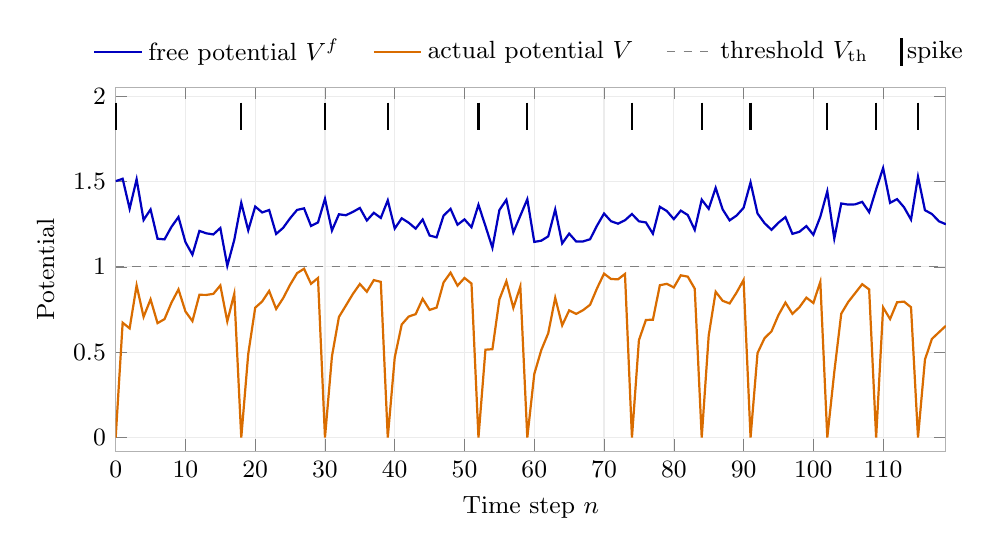
\begin{tikzpicture}
\begin{axis}[
  width=\textwidth, height=6.2cm,
  xmin=0, xmax=119, ymin=-0.08, ymax=2.05,
  xlabel={Time step $n$}, ylabel={Potential},
  tick label style={font=\small}, label style={font=\small},
  legend style={font=\small, draw=none, at={(0.5,1.03)}, anchor=south, /tikz/every even column/.append style={column sep=10pt}},
  legend columns=4, axis line style={gray!60}, grid=major, grid style={gray!15},
]
\addplot[thick, blue!75!black] coordinates {(0,1.5016) (1,1.5156) (2,1.3404) (3,1.5125) (4,1.2740) (5,1.3360) (6,1.1643) (7,1.1606) (8,1.2342) (9,1.2915) (10,1.1445) (11,1.0712) (12,1.2102) (13,1.1961) (14,1.1895) (15,1.2272) (16,1.0057) (17,1.1579) (18,1.3747) (19,1.2135) (20,1.3527) (21,1.3184) (22,1.3326) (23,1.1925) (24,1.2279) (25,1.2842) (26,1.3331) (27,1.3423) (28,1.2391) (29,1.2600) (30,1.3980) (31,1.2125) (32,1.3076) (33,1.3020) (34,1.3216) (35,1.3446) (36,1.2714) (37,1.3164) (38,1.2862) (39,1.3893) (40,1.2243) (41,1.2842) (42,1.2582) (43,1.2235) (44,1.2771) (45,1.1830) (46,1.1726) (47,1.3000) (48,1.3393) (49,1.2467) (50,1.2775) (51,1.2316) (52,1.3633) (53,1.2390) (54,1.1117) (55,1.3325) (56,1.3925) (57,1.2015) (58,1.2993) (59,1.3957) (60,1.1458) (61,1.1529) (62,1.1783) (63,1.3356) (64,1.1371) (65,1.1945) (66,1.1484) (67,1.1488) (68,1.1614) (69,1.2416) (70,1.3119) (71,1.2669) (72,1.2526) (73,1.2726) (74,1.3091) (75,1.2665) (76,1.2597) (77,1.1940) (78,1.3514) (79,1.3266) (80,1.2794) (81,1.3290) (82,1.3032) (83,1.2162) (84,1.3932) (85,1.3396) (86,1.4621) (87,1.3361) (88,1.2720) (89,1.3002) (90,1.3454) (91,1.4942) (92,1.3120) (93,1.2558) (94,1.2165) (95,1.2583) (96,1.2911) (97,1.1930) (98,1.2050) (99,1.2385) (100,1.1875) (101,1.2933) (102,1.4422) (103,1.1657) (104,1.3710) (105,1.3642) (106,1.3658) (107,1.3804) (108,1.3199) (109,1.4537) (110,1.5787) (111,1.3746) (112,1.3964) (113,1.3486) (114,1.2766) (115,1.5276) (116,1.3314) (117,1.3091) (118,1.2666) (119,1.2492)};
\addlegendentry{free potential $V^f$}
\addplot[thick, orange!85!black] coordinates {(0,0.0000) (1,0.6726) (2,0.6394) (3,0.8911) (4,0.7066) (5,0.8092) (6,0.6701) (7,0.6935) (8,0.7902) (9,0.8677) (10,0.7385) (11,0.6818) (12,0.8359) (13,0.8354) (14,0.8415) (15,0.8907) (16,0.6801) (17,0.8424) (18,0.0000) (19,0.4895) (20,0.7605) (21,0.7970) (22,0.8584) (23,0.7531) (24,0.8158) (25,0.8946) (26,0.9627) (27,0.9886) (28,0.9003) (29,0.9344) (30,0.0000) (31,0.4761) (32,0.7061) (33,0.7733) (34,0.8410) (35,0.8993) (36,0.8540) (37,0.9220) (38,0.9118) (39,0.0000) (40,0.4696) (41,0.6619) (42,0.7087) (43,0.7227) (44,0.8126) (45,0.7474) (46,0.7609) (47,0.9086) (48,0.9657) (49,0.8894) (50,0.9347) (51,0.9020) (52,0.0000) (53,0.5143) (54,0.5175) (55,0.8090) (56,0.9158) (57,0.7593) (58,0.8845) (59,0.0000) (60,0.3721) (61,0.5117) (62,0.6109) (63,0.8181) (64,0.6570) (65,0.7448) (66,0.7240) (67,0.7461) (68,0.7776) (69,0.8745) (70,0.9599) (71,0.9286) (72,0.9267) (73,0.9581) (74,0.0000) (75,0.5704) (76,0.6885) (77,0.6902) (78,0.8921) (79,0.9002) (80,0.8791) (81,0.9500) (82,0.9424) (83,0.8719) (84,0.0000) (85,0.5974) (86,0.8539) (87,0.8009) (88,0.7853) (89,0.8493) (90,0.9229) (91,0.0000) (92,0.4947) (93,0.5817) (94,0.6218) (95,0.7175) (96,0.7906) (97,0.7246) (98,0.7631) (99,0.8193) (100,0.7881) (101,0.9113) (102,0.0000) (103,0.3832) (104,0.7256) (105,0.7940) (106,0.8460) (107,0.8981) (108,0.8674) (109,0.0000) (110,0.7617) (111,0.6940) (112,0.7921) (113,0.7961) (114,0.7632) (115,0.0000) (116,0.4571) (117,0.5779) (118,0.6165) (119,0.6547)};
\addlegendentry{actual potential $V$}
\addplot[dashed, gray] coordinates {(0,1) (119,1)};
\addlegendentry{threshold $V_{\mathrm{th}}$}
\addplot[only marks, mark=|, mark size=5pt, black, thick] coordinates {(0,1.88) (18,1.88) (30,1.88) (39,1.88) (52,1.88) (59,1.88) (74,1.88) (84,1.88) (91,1.88) (102,1.88) (109,1.88) (115,1.88)};
\addlegendentry{spike}
\end{axis}
\end{tikzpicture}
\caption{The actual potential $V$ and the free potential $V^f$ of the same neuron, driven by the same input ($\mu = 0.22$). $V$ drops to the reset value at each spike and is pulled back toward its past values on the next step. $V^f$ never resets; it is the input passed through the neuron's filter, and it stays above threshold here because the mean input exceeds the rheobase.}
\label{fig:trace}
\end{figure}

%=====================================================================
\section{Step 1: the free potential}
\label{sec:free}

The \emph{free potential} $V^f$ is what the potential would be if the threshold and reset were switched off. It obeys the same update, Eq.~\eqref{eq:glflif}, with the same input $I_n$, and nothing else:
\begin{equation}
V^f_n = \Delta t^{\alpha}\left( -\frac{V^f_{n-1} - \Vrest}{\tau_m} + I_n + b \right) - \sum_{k=1}^{L} c_k\, V^f_{n-k}.
\label{eq:vfree}
\end{equation}
This is a linear difference equation with constant coefficients, so $V^f$ is a \emph{linear filter} of the input. If the input is a sum $I = I^{(1)} + I^{(2)}$, the free potential is the sum of the free potentials each part would produce. (The constant terms $\Vrest/\tau_m + b$ can be treated as part of the input.) The jumps of obstacle~2 are gone.

Two remarks keep this in perspective.
\begin{itemize}
  \item $V^f$ is computed alongside the real network. It is driven by the real spikes of the other neurons through Eq.~\eqref{eq:input}, and it does not change the network. It is a bookkeeping variable, and you can compute it from a recorded run.
  \item $V$ and $V^f$ differ only by the effect of past resets. Each reset removes some potential, and that removal is then carried forward by the same linear filter. Section~9 of the main document writes this as an exact identity. In Figure~\ref{fig:trace}, $V$ sits about 0.4 to 0.6 below $V^f$ between spikes: that gap is the accumulated reset deficit.
\end{itemize}

%=====================================================================
\section{Step 2: the operating point}
\label{sec:operating}

A tangent line needs a point of tangency. Here that point is the neuron's \emph{operating point}: its average behaviour when the network is running normally. It has three parts.

\begin{itemize}
  \item The \emph{mean input} $\bar I_j$, the time average of $I_{j,n}$.
  \item The \emph{mean rate} $r_j$, the time average of $s_{j,n}$, in spikes per step. Since $s_{j,n}$ is 0 or 1, $r_j$ is also the probability of a spike in a given step.
  \item The \emph{mean free potential} $\bar V_j$, the time average of $V^f_{j,n}$.
\end{itemize}

\paragraph{The mean free potential from the mean input.} For a constant input $\bar I$, Eq.~\eqref{eq:vfree} settles to a constant $\bar V$ (assuming the filter is stable). Substituting $V^f_n = \bar V$ for every $n$:
\begin{equation*}
\bar V = \Delta t^{\alpha}\left( -\frac{\bar V - \Vrest}{\tau_m} + \bar I + b \right) - \Big( \sum_{k=1}^{L} c_k \Big) \bar V.
\end{equation*}
By Eq.~\eqref{eq:epsL}, $\sum_{k=1}^{L} c_k = \varepsilon_L - 1$, so the $\bar V$ terms combine to $\varepsilon_L \bar V$ on the left. Dividing by $\Delta t^{\alpha}$ and collecting:
\begin{equation}
\bar V = \GDC \left( \frac{\Vrest}{\tau_m} + \bar I + b \right), \qquad \GDC = \left( \frac{1}{\tau_m} + \frac{\varepsilon_L}{\Delta t^{\alpha}} \right)^{-1}.
\label{eq:gdc}
\end{equation}
$\GDC$ is the \emph{DC gain} of the filter: a constant change $\Delta I$ in the input moves the free potential by $\GDC\,\Delta I$. With the full history, $\varepsilon_L = 0$ and $\GDC = \tau_m$, the same as the integer-order neuron: a fractional derivative of a constant is zero, so the order $\alpha$ does not change where the neuron settles. With truncation, $\varepsilon_L$ adds leak. For the simulated neuron, $\GDC = (0.1 + 0.070)^{-1} = 5.87$ instead of 10. Because Eq.~\eqref{eq:vfree} is linear, the time average of $V^f$ obeys Eq.~\eqref{eq:gdc} even when the input fluctuates. In the simulation with $\mu = 0.22$, the measured mean of $V^f$ is 1.2912 and $\GDC \mu = 1.2912$.

%=====================================================================
\section{Step 3: a smooth spike response}
\label{sec:smooth}

\subsection{Averaging turns a step into a smooth curve}

Obstacle~1 disappears once we stop asking whether a spike happens and ask how \emph{often} it happens. A one-line calculation shows why averaging helps. Suppose that at some step the potential is $v + \xi$, where $v$ is fixed and $\xi$ is random noise with density $p$ and cumulative distribution $F$. The expected output is
\begin{equation*}
\E[s] = \E\big[ H(v + \xi - \Vth) \big] = \Pr(\xi \ge \Vth - v) = 1 - F(\Vth - v),
\qquad \frac{d\,\E[s]}{dv} = p(\Vth - v).
\end{equation*}
The step function has become a smooth, increasing curve whose slope is the noise density. For Gaussian noise of standard deviation $\sigma$ it is the normal CDF, with maximum slope $1/(\sigma\sqrt{2\pi})$ at threshold. As $\sigma \to 0$ the curve steepens back into the step. The same idea applies over time: a neuron in a driven network sees a fluctuating input, and its \emph{average} output is a smooth function of its \emph{average} input.

\subsection{The \texorpdfstring{$f$--$I$}{f-I} curve}

The \emph{$f$--$I$ curve} $r = f(\bar I)$ gives a neuron's firing rate ($f$ for frequency) as a function of its mean input. The input level at which a noiseless neuron starts firing is the \emph{rheobase}. For the simulated neuron it is where the settled potential just reaches threshold, $\GDC\,\bar I = \Vth$, so $\bar I = 1/5.87 = 0.170$.

Without noise the curve has an infinite slope at the rheobase. For the integer-order LIF neuron this is a short calculation. Take $\Vrest = \Vreset = 0$, $b = 0$ and constant input $I > \Vth/\tau_m$. Starting from reset, $V(t) = I\tau_m(1 - e^{-t/\tau_m})$ reaches threshold at
\begin{equation*}
T(I) = \tau_m \ln \frac{I\tau_m}{I\tau_m - \Vth}, \qquad f(I) = \frac{1}{T(I)}, \qquad f'(I) = -\frac{T'(I)}{T(I)^2}.
\end{equation*}
As $I$ decreases to $\Vth/\tau_m$, $T'(I) \approx -\tau_m^2/(I\tau_m - \Vth) \to -\infty$ while $T^2$ grows only like a squared logarithm, so $f'(I) \to +\infty$. In discrete time, a noiseless neuron's period is a whole number of steps, so its rate can only take values $1/1, 1/2, 1/3, \dots$ at constant input, and its curve is a staircase. Figure~\ref{fig:fi} shows both effects, and also shows that input noise smooths them away. The main document uses this \emph{noise-averaged} curve, with the noise level a neuron actually experiences in the running network.

\begin{figure}[h]
\centering
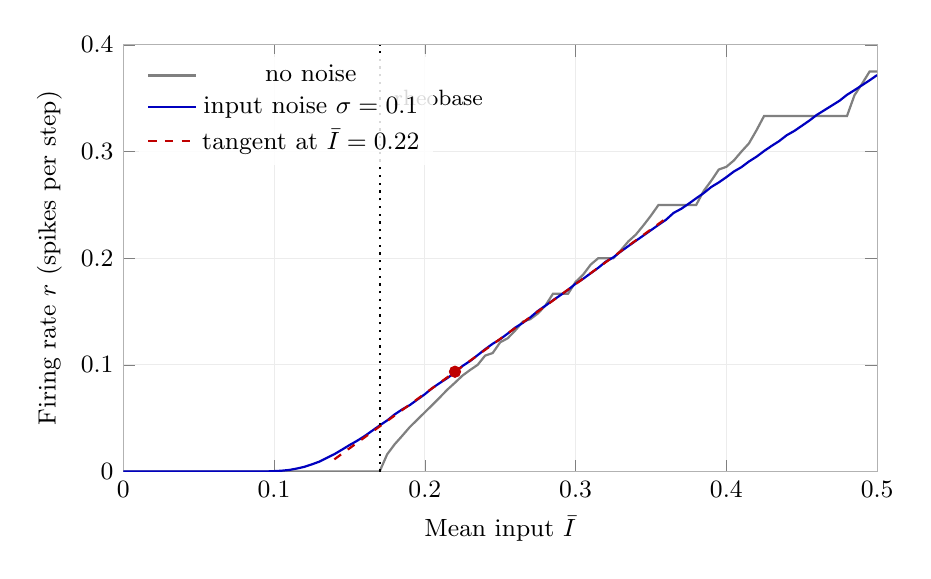
\begin{tikzpicture}
\begin{axis}[
  width=0.92\textwidth, height=7cm,
  xmin=0, xmax=0.5, ymin=0, ymax=0.4,
  xlabel={Mean input $\bar I$}, ylabel={Firing rate $r$ (spikes per step)},
  xtick={0,0.1,0.2,0.3,0.4,0.5}, scaled x ticks=false, xticklabel style={/pgf/number format/fixed},
  tick label style={font=\small}, label style={font=\small},
  legend style={font=\small, draw=none, fill=white, fill opacity=0.85, text opacity=1, at={(0.02,0.98)}, anchor=north west},
  axis line style={gray!60}, grid=major, grid style={gray!15},
]
\addplot[thick, gray] coordinates {(0.000,0.0000) (0.005,0.0000) (0.010,0.0000) (0.015,0.0000) (0.020,0.0000) (0.025,0.0000) (0.030,0.0000) (0.035,0.0000) (0.040,0.0000) (0.045,0.0000) (0.050,0.0000) (0.055,0.0000) (0.060,0.0000) (0.065,0.0000) (0.070,0.0000) (0.075,0.0000) (0.080,0.0000) (0.085,0.0000) (0.090,0.0000) (0.095,0.0000) (0.100,0.0000) (0.105,0.0000) (0.110,0.0000) (0.115,0.0000) (0.120,0.0000) (0.125,0.0000) (0.130,0.0000) (0.135,0.0000) (0.140,0.0000) (0.145,0.0000) (0.150,0.0000) (0.155,0.0000) (0.160,0.0000) (0.165,0.0000) (0.170,0.0000) (0.175,0.0161) (0.180,0.0256) (0.185,0.0335) (0.190,0.0417) (0.195,0.0486) (0.200,0.0556) (0.205,0.0625) (0.210,0.0696) (0.215,0.0769) (0.220,0.0833) (0.225,0.0900) (0.230,0.0952) (0.235,0.1000) (0.240,0.1087) (0.245,0.1111) (0.250,0.1212) (0.255,0.1250) (0.260,0.1323) (0.265,0.1405) (0.270,0.1429) (0.275,0.1482) (0.280,0.1557) (0.285,0.1667) (0.290,0.1667) (0.295,0.1667) (0.300,0.1778) (0.305,0.1846) (0.310,0.1940) (0.315,0.2000) (0.320,0.2000) (0.325,0.2000) (0.330,0.2075) (0.335,0.2158) (0.340,0.2222) (0.345,0.2308) (0.350,0.2400) (0.355,0.2500) (0.360,0.2500) (0.365,0.2500) (0.370,0.2500) (0.375,0.2500) (0.380,0.2500) (0.385,0.2632) (0.390,0.2727) (0.395,0.2832) (0.400,0.2857) (0.405,0.2917) (0.410,0.3000) (0.415,0.3077) (0.420,0.3200) (0.425,0.3333) (0.430,0.3333) (0.435,0.3333) (0.440,0.3333) (0.445,0.3333) (0.450,0.3333) (0.455,0.3333) (0.460,0.3333) (0.465,0.3333) (0.470,0.3333) (0.475,0.3333) (0.480,0.3333) (0.485,0.3529) (0.490,0.3636) (0.495,0.3750) (0.500,0.3750)};
\addlegendentry{no noise}
\addplot[thick, blue!75!black] coordinates {(0.000,0.0000) (0.005,0.0000) (0.010,0.0000) (0.015,0.0000) (0.020,0.0000) (0.025,0.0000) (0.030,0.0000) (0.035,0.0000) (0.040,0.0000) (0.045,0.0000) (0.050,0.0000) (0.055,0.0000) (0.060,0.0000) (0.065,0.0000) (0.070,0.0000) (0.075,0.0000) (0.080,0.0000) (0.085,0.0000) (0.090,0.0001) (0.095,0.0001) (0.100,0.0004) (0.105,0.0008) (0.110,0.0015) (0.115,0.0028) (0.120,0.0044) (0.125,0.0067) (0.130,0.0093) (0.135,0.0128) (0.140,0.0163) (0.145,0.0205) (0.150,0.0248) (0.155,0.0288) (0.160,0.0332) (0.165,0.0382) (0.170,0.0432) (0.175,0.0479) (0.180,0.0536) (0.185,0.0583) (0.190,0.0623) (0.195,0.0674) (0.200,0.0725) (0.205,0.0783) (0.210,0.0831) (0.215,0.0877) (0.220,0.0929) (0.225,0.0990) (0.230,0.1036) (0.235,0.1091) (0.240,0.1147) (0.245,0.1198) (0.250,0.1241) (0.255,0.1294) (0.260,0.1350) (0.265,0.1394) (0.270,0.1446) (0.275,0.1506) (0.280,0.1555) (0.285,0.1606) (0.290,0.1654) (0.295,0.1704) (0.300,0.1761) (0.305,0.1807) (0.310,0.1859) (0.315,0.1910) (0.320,0.1968) (0.325,0.2008) (0.330,0.2063) (0.335,0.2114) (0.340,0.2164) (0.345,0.2213) (0.350,0.2263) (0.355,0.2313) (0.360,0.2361) (0.365,0.2425) (0.370,0.2463) (0.375,0.2511) (0.380,0.2562) (0.385,0.2611) (0.390,0.2668) (0.395,0.2711) (0.400,0.2760) (0.405,0.2813) (0.410,0.2854) (0.415,0.2907) (0.420,0.2952) (0.425,0.3005) (0.430,0.3053) (0.435,0.3098) (0.440,0.3153) (0.445,0.3193) (0.450,0.3241) (0.455,0.3290) (0.460,0.3344) (0.465,0.3388) (0.470,0.3432) (0.475,0.3476) (0.480,0.3532) (0.485,0.3576) (0.490,0.3622) (0.495,0.3668) (0.500,0.3717)};
\addlegendentry{input noise $\sigma = 0.1$}
\addplot[thick, dashed, red!75!black, domain=0.14:0.36, samples=2] {0.0936 + 1.0266*(x - 0.22)};
\addlegendentry{tangent at $\bar I = 0.22$}
\addplot[only marks, mark=*, mark size=2pt, red!75!black, forget plot] coordinates {(0.22,0.0936)};
\addplot[dotted, thick, black, forget plot] coordinates {(0.1704,0) (0.1704,0.4)};
\node[anchor=west, font=\footnotesize] at (axis cs:0.173,0.35) {rheobase};
\end{axis}
\end{tikzpicture}
\caption{Firing rate against mean input for the simulated neuron. Without noise the curve is a staircase that starts abruptly at the rheobase. With input noise it is smooth, and above the rheobase it is nearly straight: the tangent line at $\bar I = 0.22$ stays within a few percent of it from 0.16 up to the edge of the plot. Below the rheobase the rate tails off toward zero and the tangent fails.}
\label{fig:fi}
\end{figure}

\subsection{The tangent line, in units of the free potential}

The slope $f'(\bar I_j)$ of the noise-averaged curve is the \emph{$f$--$I$ gain}: extra spikes per step per unit of extra mean input. The linear model is written in terms of the free potential rather than the input, so the slope has to be converted. By Eq.~\eqref{eq:gdc}, $d\bar V_j / d\bar I_j = \GDC$, and the chain rule gives the gain per unit of free potential:
\begin{equation}
\gamma_j = \frac{dr_j}{d\bar V_j} = \frac{dr_j/d\bar I_j}{d\bar V_j/d\bar I_j} = \frac{f_j'(\bar I_j)}{\GDC}.
\label{eq:gamma}
\end{equation}
The first-order Taylor expansion of the spike output around the operating point is then
\begin{equation}
s_{j,n} \approx r_j + \gamma_j \left( V^f_{j,n} - \bar V_j \right).
\label{eq:spikelin}
\end{equation}
This is the linearization of the main document. Three things about it are easy to miss.

\begin{itemize}
  \item \textbf{The ``$\approx$'' is about averages.} The left side is 0 or 1. The right side is a smooth number near $r_j$. What Eq.~\eqref{eq:spikelin} claims is that the right side is the neuron's expected output. The actual output equals it plus a zero-mean ``spike noise'' that the linear model drops.
  \item \textbf{$\gamma_j$ is a slow, or DC, gain.} It was computed from mean input against mean rate, so it describes how the rate follows \emph{slow} changes in $V^f$. Section~\ref{sec:measure} shows that fast changes get through more strongly.
  \item \textbf{Silent neurons drop out.} A neuron far below its rheobase has $r_j = 0$ and $\gamma_j = 0$. It sends nothing, and the linear model ignores it. A neuron just below its rheobase has a small but nonzero $\gamma_j$ on the noise-averaged curve, and a fault elsewhere can push it into firing.
\end{itemize}

%=====================================================================
\section{Measuring \texorpdfstring{$r_j$, $\gamma_j$ and $\bar V_j$}{the operating point}}
\label{sec:measure}

\paragraph{The mean rate and mean free potential} are plain time averages over a recorded fault-free run, after discarding the initial transient. $\bar V_j$ needs $V^f_j$, which is obtained by replaying the recorded input $I_{j,n}$ through Eq.~\eqref{eq:vfree}.

\paragraph{The gain by sweeping the mean.} This is a numerical derivative. Drive a single copy of the neuron with input $\mu + (\text{noise})$, with the noise matched to what neuron $j$ sees, and measure the rate at $\mu = \bar I_j \pm h$. The central difference
\begin{equation*}
f'(\bar I_j) \approx \frac{f(\bar I_j + h) - f(\bar I_j - h)}{2h}
\end{equation*}
then gives $\gamma_j$ through Eq.~\eqref{eq:gamma}. The usual finite-difference trade-off applies. If $h$ is too small, the statistical noise in the measured rates swamps the difference. If $h$ is too large, the curvature of $f$ biases it. For the simulated neuron at $\bar I = 0.22$, $h = 0.02$ gives $f' = 1.027$ and $\gamma = 1.027/5.87 = 0.175$.

\paragraph{The gain depends on how fast the input changes.} To check that 0.175 is right, drive the neuron with $\mu(t) = 0.22 + 0.02\sin(2\pi t/P)$ plus the same noise, and measure how much the rate oscillates per unit of oscillation in $V^f$. Figure~\ref{fig:gain} shows the result against frequency $1/P$. For slow oscillations, with periods of a thousand steps or more, the gain is close to 0.176, matching Eq.~\eqref{eq:gamma}. For faster oscillations it is larger: twice as large at a period of 100 steps, and seven times as large at 10 steps.

The reason is the reset. When $V^f$ rises slowly, the neuron fires more, and every extra spike's reset lowers $V$ for a long time afterwards, through the same memory. That suppresses further spikes and cancels much of the increase. When $V^f$ rises briefly, the extra spikes happen before the cancellation catches up. A fractional neuron spreads the cancellation over its long memory, so its gain changes over a much wider range of frequencies than an integer-order neuron's. In Figure~\ref{fig:gain} the $\alpha = 1$ neuron is flat down to periods of about 300 steps, and the $\alpha = 0.5$ neuron is not.

\begin{figure}[h]
\centering
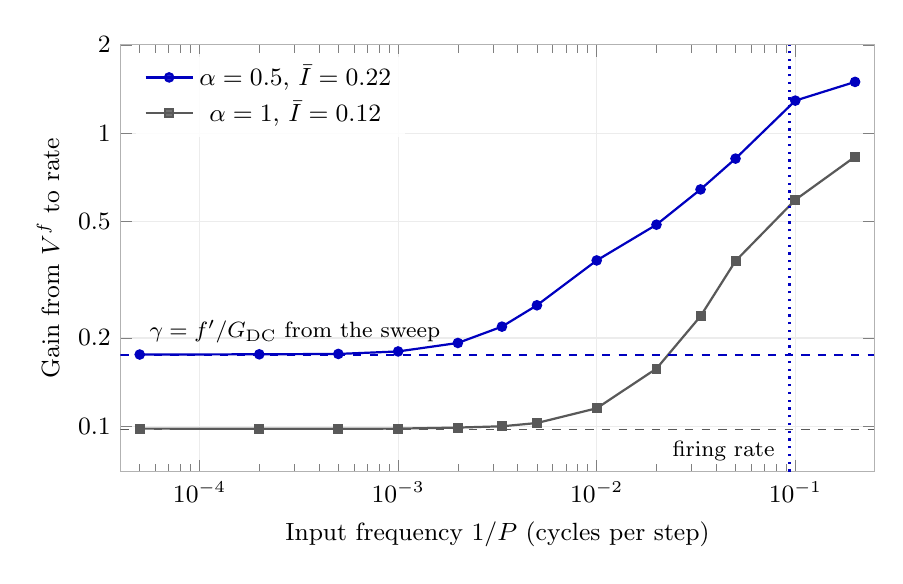
\begin{tikzpicture}
\begin{loglogaxis}[
  width=0.92\textwidth, height=7cm,
  xmin=4e-5, xmax=0.25, ymin=0.07, ymax=2,
  xlabel={Input frequency $1/P$ (cycles per step)}, ylabel={Gain from $V^f$ to rate},
  ytick={0.1,0.2,0.5,1,2}, yticklabels={0.1,0.2,0.5,1,2},
  tick label style={font=\small}, label style={font=\small},
  legend style={font=\small, draw=none, fill=white, fill opacity=0.85, text opacity=1, at={(0.02,0.98)}, anchor=north west},
  axis line style={gray!60}, grid=major, grid style={gray!15},
]
\addplot[thick, blue!75!black, mark=*, mark size=1.5pt] coordinates {(5e-05,0.1756) (0.0002,0.1759) (0.0005,0.1764) (0.001,0.1799) (0.002,0.1923) (0.00333333,0.2186) (0.005,0.2585) (0.01,0.3678) (0.02,0.4871) (0.0333333,0.6426) (0.05,0.8186) (0.1,1.2910) (0.2,1.4957)};
\addlegendentry{$\alpha = 0.5$, $\bar I = 0.22$}
\addplot[thick, gray!70!black, mark=square*, mark size=1.4pt] coordinates {(5e-05,0.0981) (0.0002,0.0980) (0.0005,0.0980) (0.001,0.0981) (0.002,0.0989) (0.00333333,0.0999) (0.005,0.1025) (0.01,0.1151) (0.02,0.1572) (0.0333333,0.2373) (0.05,0.3662) (0.1,0.5920) (0.2,0.8309)};
\addlegendentry{$\alpha = 1$, $\bar I = 0.12$}
\addplot[dashed, blue!75!black, forget plot] coordinates {(4e-5,0.1749) (0.25,0.1749)};
\addplot[dashed, gray!70!black, forget plot] coordinates {(4e-5,0.0976) (0.25,0.0976)};
\addplot[dotted, thick, blue!75!black, forget plot] coordinates {(0.0936,0.07) (0.0936,2)};
\node[anchor=south west, font=\footnotesize] at (axis cs:5e-5,0.178) {$\gamma = f'/G_{\mathrm{DC}}$ from the sweep};
\node[anchor=east, font=\footnotesize] at (axis cs:0.088,0.082) {firing rate};
\end{loglogaxis}
\end{tikzpicture}
\caption{How strongly the firing rate follows an oscillation in the free potential, against the oscillation's frequency. Dashed lines: the slow gain $\gamma$ of Eq.~\eqref{eq:gamma}, measured by sweeping the mean input. The measured gain matches it for slow oscillations and grows for fast ones, well below the firing rate (dotted, for $\alpha = 0.5$).}
\label{fig:gain}
\end{figure}

\paragraph{The gain by regression, and why it differs.} The main document also suggests a second method: regress the recorded spikes on the free potential and take the slope,
\begin{equation*}
\hat\gamma_j = \frac{\Cov(s_j, V^f_j)}{\Var(V^f_j)},
\end{equation*}
which is the slope of the best-fitting straight line through the points $(V^f_{j,n}, s_{j,n})$. It is cheap, because it needs only a recorded run. But it weights each frequency by how much of it is present in $V^f$, and a neuron driven by fluctuating input has plenty of fast fluctuation. In the simulation the regression gives $\hat\gamma = 0.84$ for $\alpha = 0.5$, against the slow gain 0.175, and 0.19 against 0.098 for $\alpha = 1$. So the step-by-step regression measures a different, faster gain, not $\gamma_j$ of Eq.~\eqref{eq:gamma}.

\paragraph{The gain by windowed regression.} The fix is to remove the fast fluctuations before regressing. Split the recorded run into consecutive windows of $W$ steps, average $s_j$ and $V^f_j$ over each window, and regress the window averages on each other. Averaging over a window is a low-pass filter, so only fluctuations slower than about $W$ steps survive, and Figure~\ref{fig:gain} says those are exactly the ones whose gain is $\gamma_j$. In the simulation, with $\alpha = 0.5$, the slope falls from 0.84 at $W = 1$ to 0.19 at $W = 100$ and 0.1765 at $W = 1000$, against $\gamma = 0.175$ from the sweep. For $\alpha = 1$, $W = 100$ already gives 0.099 against 0.098. A recorded run of $2 \times 10^{5}$ steps, which is 200 windows of 1000 steps, gave estimates within about 5\% of $\gamma$. This is the golden-run method the main document recommends. It needs no extra experiment, and on hardware it automatically includes truncation and quantization.

%=====================================================================
\section{Step 4: assembling the linear network}
\label{sec:assemble}

\subsection{One neuron's equation}

Insert the linearized spikes, Eq.~\eqref{eq:spikelin}, into neuron $i$'s input, Eq.~\eqref{eq:input}. Because spikes arrive one step late, the linearization is applied at step $n-1$:
\begin{equation*}
\sum_j W_{ij}\, s_{j,n-1} \approx \sum_j W_{ij}\gamma_j\, V^f_{j,n-1} + \sum_j W_{ij}\left( r_j - \gamma_j \bar V_j \right).
\end{equation*}
The first sum depends on the other neurons' free potentials. The second is a constant. Substituting into the free-potential update, Eq.~\eqref{eq:vfree}, and splitting the leak as $-(V^f_{i,n-1} - \Vrest)/\tau_m = -V^f_{i,n-1}/\tau_m + \Vrest/\tau_m$ gives, inside the parentheses,
\begin{equation*}
\underbrace{-\frac{V^f_{i,n-1}}{\tau_m} + \sum_j W_{ij}\gamma_j\, V^f_{j,n-1}}_{\text{previous free potentials}}
\;+\; \underbrace{\sum_m W^{\mathrm{in}}_{im}\, u_{m,n}}_{\text{external input}}
\;+\; \underbrace{\frac{\Vrest}{\tau_m} + b + \sum_j W_{ij}\left( r_j - \gamma_j \bar V_j \right)}_{\text{constant}}.
\end{equation*}
Every term is now either a constant or a linear function of free potentials and inputs. Neuron $i$ no longer needs anyone's spikes, only their free potentials.

\subsection{A two-neuron example}

For two neurons connected to each other but not to themselves, with $W = \left(\begin{smallmatrix} 0 & W_{12} \\ W_{21} & 0 \end{smallmatrix}\right)$, the two equations are
\begin{align*}
V^f_{1,n} &= \Delta t^{\alpha}\left( -\tfrac{1}{\tau_m} V^f_{1,n-1} + W_{12}\gamma_2\, V^f_{2,n-1} + \textstyle\sum_m W^{\mathrm{in}}_{1m} u_{m,n} + \beta_1 \right) - \textstyle\sum_{k=1}^{L} c_k V^f_{1,n-k}, \\
V^f_{2,n} &= \Delta t^{\alpha}\left( W_{21}\gamma_1\, V^f_{1,n-1} - \tfrac{1}{\tau_m} V^f_{2,n-1} + \textstyle\sum_m W^{\mathrm{in}}_{2m} u_{m,n} + \beta_2 \right) - \textstyle\sum_{k=1}^{L} c_k V^f_{2,n-k},
\end{align*}
with constants $\beta_1 = \Vrest/\tau_m + b + W_{12}(r_2 - \gamma_2 \bar V_2)$ and $\beta_2 = \Vrest/\tau_m + b + W_{21}(r_1 - \gamma_1 \bar V_1)$. The coefficients of the previous free potentials form the matrix
\begin{equation*}
A = \begin{pmatrix} -1/\tau_m & W_{12}\gamma_2 \\ W_{21}\gamma_1 & -1/\tau_m \end{pmatrix}
= -\frac{1}{\tau_m}\,\mathrm{Id} + \underbrace{\begin{pmatrix} 0 & W_{12} \\ W_{21} & 0 \end{pmatrix}\begin{pmatrix} \gamma_1 & 0 \\ 0 & \gamma_2 \end{pmatrix}}_{\Wt \;=\; W\,\mathrm{diag}(\gamma)}.
\end{equation*}
Each column of $W$ is scaled by the gain of the neuron that sends along it: a connection from a neuron that barely responds carries almost nothing.

\subsection{The general form}

Stack the free potentials into a vector $x_n = (V^f_{1,n}, \dots, V^f_{N,n})$. The coefficients $c_k$ are the same numbers for every neuron, so the memory sum stacks directly, and the $N$ equations become one:
\begin{equation}
\begin{gathered}
x_n = \Delta t^{\alpha}\left( A\, x_{n-1} + B\, u_n + \beta \right) - \sum_{k=1}^{L} c_k\, x_{n-k}, \\
A = -\tfrac{1}{\tau_m}\mathrm{Id} + \Wt, \quad \Wt = W\,\mathrm{diag}(\gamma), \quad B = W^{\mathrm{in}}, \quad
\beta = \left( \tfrac{\Vrest}{\tau_m} + b \right)\mathbf{1} + W\left( r - \mathrm{diag}(\gamma)\,\bar V \right),
\end{gathered}
\label{eq:linfor}
\end{equation}
where $\mathbf{1}$ is the all-ones vector. This is the \emph{linear fractional-order reservoir} (linear FOR) of the main document. As $\Delta t \to 0$ with the memory $L\Delta t \to \infty$, the left side becomes a GL derivative and Eq.~\eqref{eq:linfor} becomes $D^{\alpha} x = A x + B u + \beta$. Everything the main document derives (fault responses, recovery times, stability) comes from the eigenvalues of $A$ and this one equation.

%=====================================================================
\section{When can the approximation be trusted?}
\label{sec:accuracy}

The only approximation is Eq.~\eqref{eq:spikelin}. Everything after it is exact algebra. Eq.~\eqref{eq:spikelin} can fail in four ways.

\begin{itemize}
  \item \textbf{Too large a change.} A tangent line is accurate only where the curve is nearly straight. In Figure~\ref{fig:fi} the noisy curve is nearly straight above the rheobase, so the tangent at $\bar I = 0.22$ stays within a few percent of it from 0.16 upward. Below the rheobase the rate tails off toward zero, and the tangent is 30\% off at 0.14. For a fault, the relevant change is the shift in mean input that the fault causes, $-W_{ij} r_j$ for a target of a removed neuron $j$. It must not carry the neuron across that bend.
  \item \textbf{Too fast a change.} As Figure~\ref{fig:gain} shows, a single static $\gamma_j$ is right for slow changes and too small for fast ones. Results about slow quantities, such as the shift in mean operating point after a permanent fault, are safest. Results that depend on fluctuations at all frequencies, such as memory capacity and information measures, inherit an error from the frequency dependence of the gain, and that error is larger at low $\alpha$.
  \item \textbf{Spike noise.} The linear model keeps the expected output and drops the 0/1 fluctuations around it. In the full network those fluctuations act as extra noise on every neuron.
  \item \textbf{Neurons that switch on or off.} The tangent line of a silent neuron is flat, so the linear model cannot predict a fault pushing it across its rheobase. Section~6 of the main document treats these switches separately.
\end{itemize}
Each of these can be checked from simulation. Compare the linear model's prediction with the spiking network's response to the same fault, and look at which of the four mechanisms explains the difference.

%=====================================================================
\section*{Symbols}
\addcontentsline{toc}{section}{Symbols}

\begin{center}
\small
\begin{tabularx}{\textwidth}{@{}l>{\raggedright\arraybackslash}X@{}}
\toprule
Symbol & Meaning \\
\midrule
$V_{i,n}$ & actual membrane potential of neuron $i$ at step $n$ (resets at each spike) \\
$V^f_{i,n}$, $x_n$ & free potential (no threshold or reset); $x_n$ is the vector of all of them \\
$s_{i,n}$ & spike output, 0 or 1 \\
$I_{i,n}$, $u_{m,n}$ & input current of neuron $i$; external input signal $m$ \\
$\tau_m$, $\Vrest$, $b$ & leak time constant, resting potential, bias \\
$\Vth$, $\Vreset$ & threshold and reset potentials \\
$\alpha$, $c_k$, $L$ & fractional order, GL coefficients $(-1)^k\binom{\alpha}{k}$, memory length \\
$\varepsilon_L$ & weight lost by keeping only $L$ past values; acts as extra leak \\
$\GDC$ & DC gain of the membrane filter, $(1/\tau_m + \varepsilon_L/\Delta t^{\alpha})^{-1}$ \\
$W$, $W^{\mathrm{in}}$ & recurrent and input weights; $W_{ij}$ is from neuron $j$ to neuron $i$ \\
$\bar I_j$, $r_j$, $\bar V_j$ & operating point: mean input, mean rate, mean free potential \\
$f_j$, $f_j'$ & noise-averaged $f$--$I$ curve and its slope \\
$\gamma_j$ & slow gain from free potential to rate, $f_j'(\bar I_j)/\GDC$ \\
$\Wt$, $A$, $B$, $\beta$ & matrices and constant of the linear FOR, Eq.~\eqref{eq:linfor} \\
\bottomrule
\end{tabularx}
\end{center}

\end{document}
